
\section{SERVICE ARCHITECTURE MODELS}
\label{chap:service}


%Infrastructure as a Service platforms at it's core controls various virtualization interfaces and services and allows to launch a new virtual server from given disk image at chosen host server, connect it to provided physical or virtual network and add block storage device to it. The OpenStack platform provides services that address needed to provide the very basic compute, network and storage services. The identity provider and image store  provide further services needed to provide the basic sevices.
%Nebula was the predecessor of OpenStack and was superseded because it did not scale well. The services withing OpenStack communicate through 3 various communication channels
%TCP/SQL - Services store it's state in SQL datastore
%AMQP - Service internally communicate over asychronous communication bus which .... Compute service calls network service 
%HTTP - All services expose REST APIs that allow higher level integration, control ...

This section describes modularity and complexity of OpenStack IaaS platform including core and supporting services. However, there is not so much place for detail description of all components, since the main idea is contained in Sections \ref{chap:ontology} and \ref{chap:usage}. 
The goal of this section is to show that OpenStack modules are independent services, which can be implemented in many different of ways. 

\subsection{IAAS ARCHITECTURE CORE MODELS}

OpenStack is complete Infrastructure as a Service platform. It allows to create virtual servers on virtual networks using virtual block devices.

\begin{figure}[h]
\centering
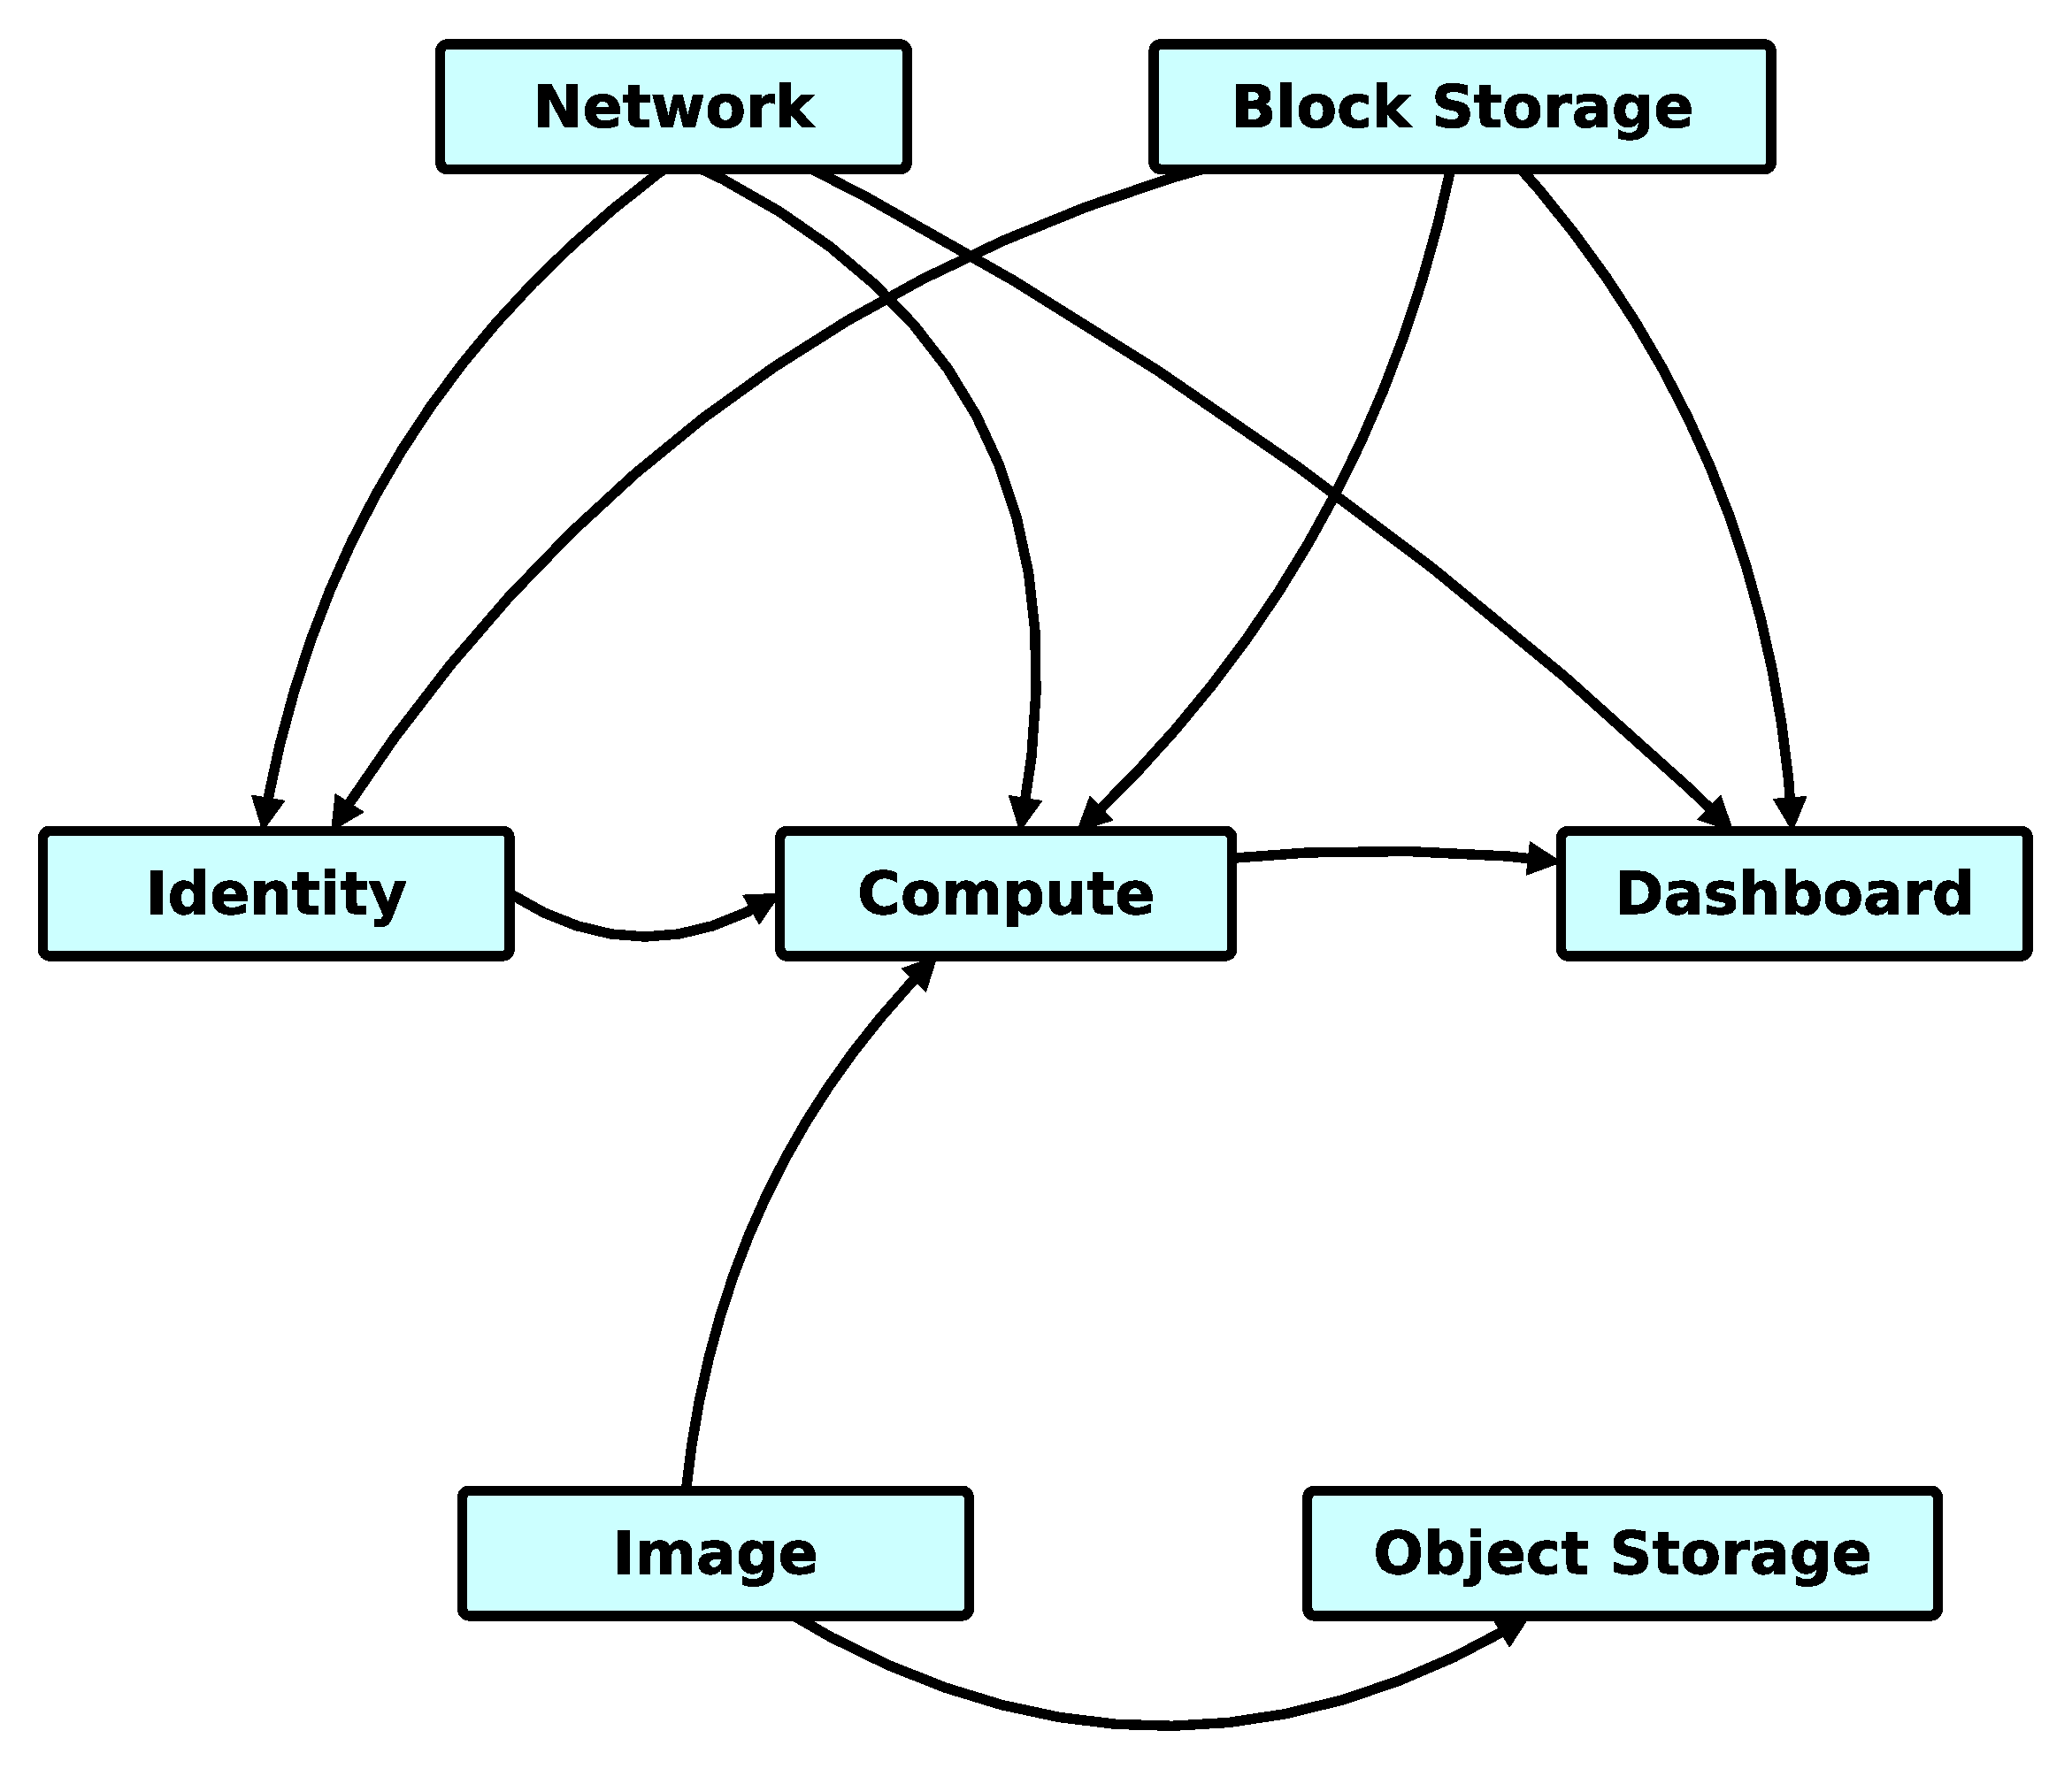
\includegraphics[scale=.13]{img/openstack_logical_model.eps}
\caption{Logical Model of Icehouse OpenStack service achitecture}
\label{fig:modules}
\end{figure}

\begin{figure}[!h]
\centering
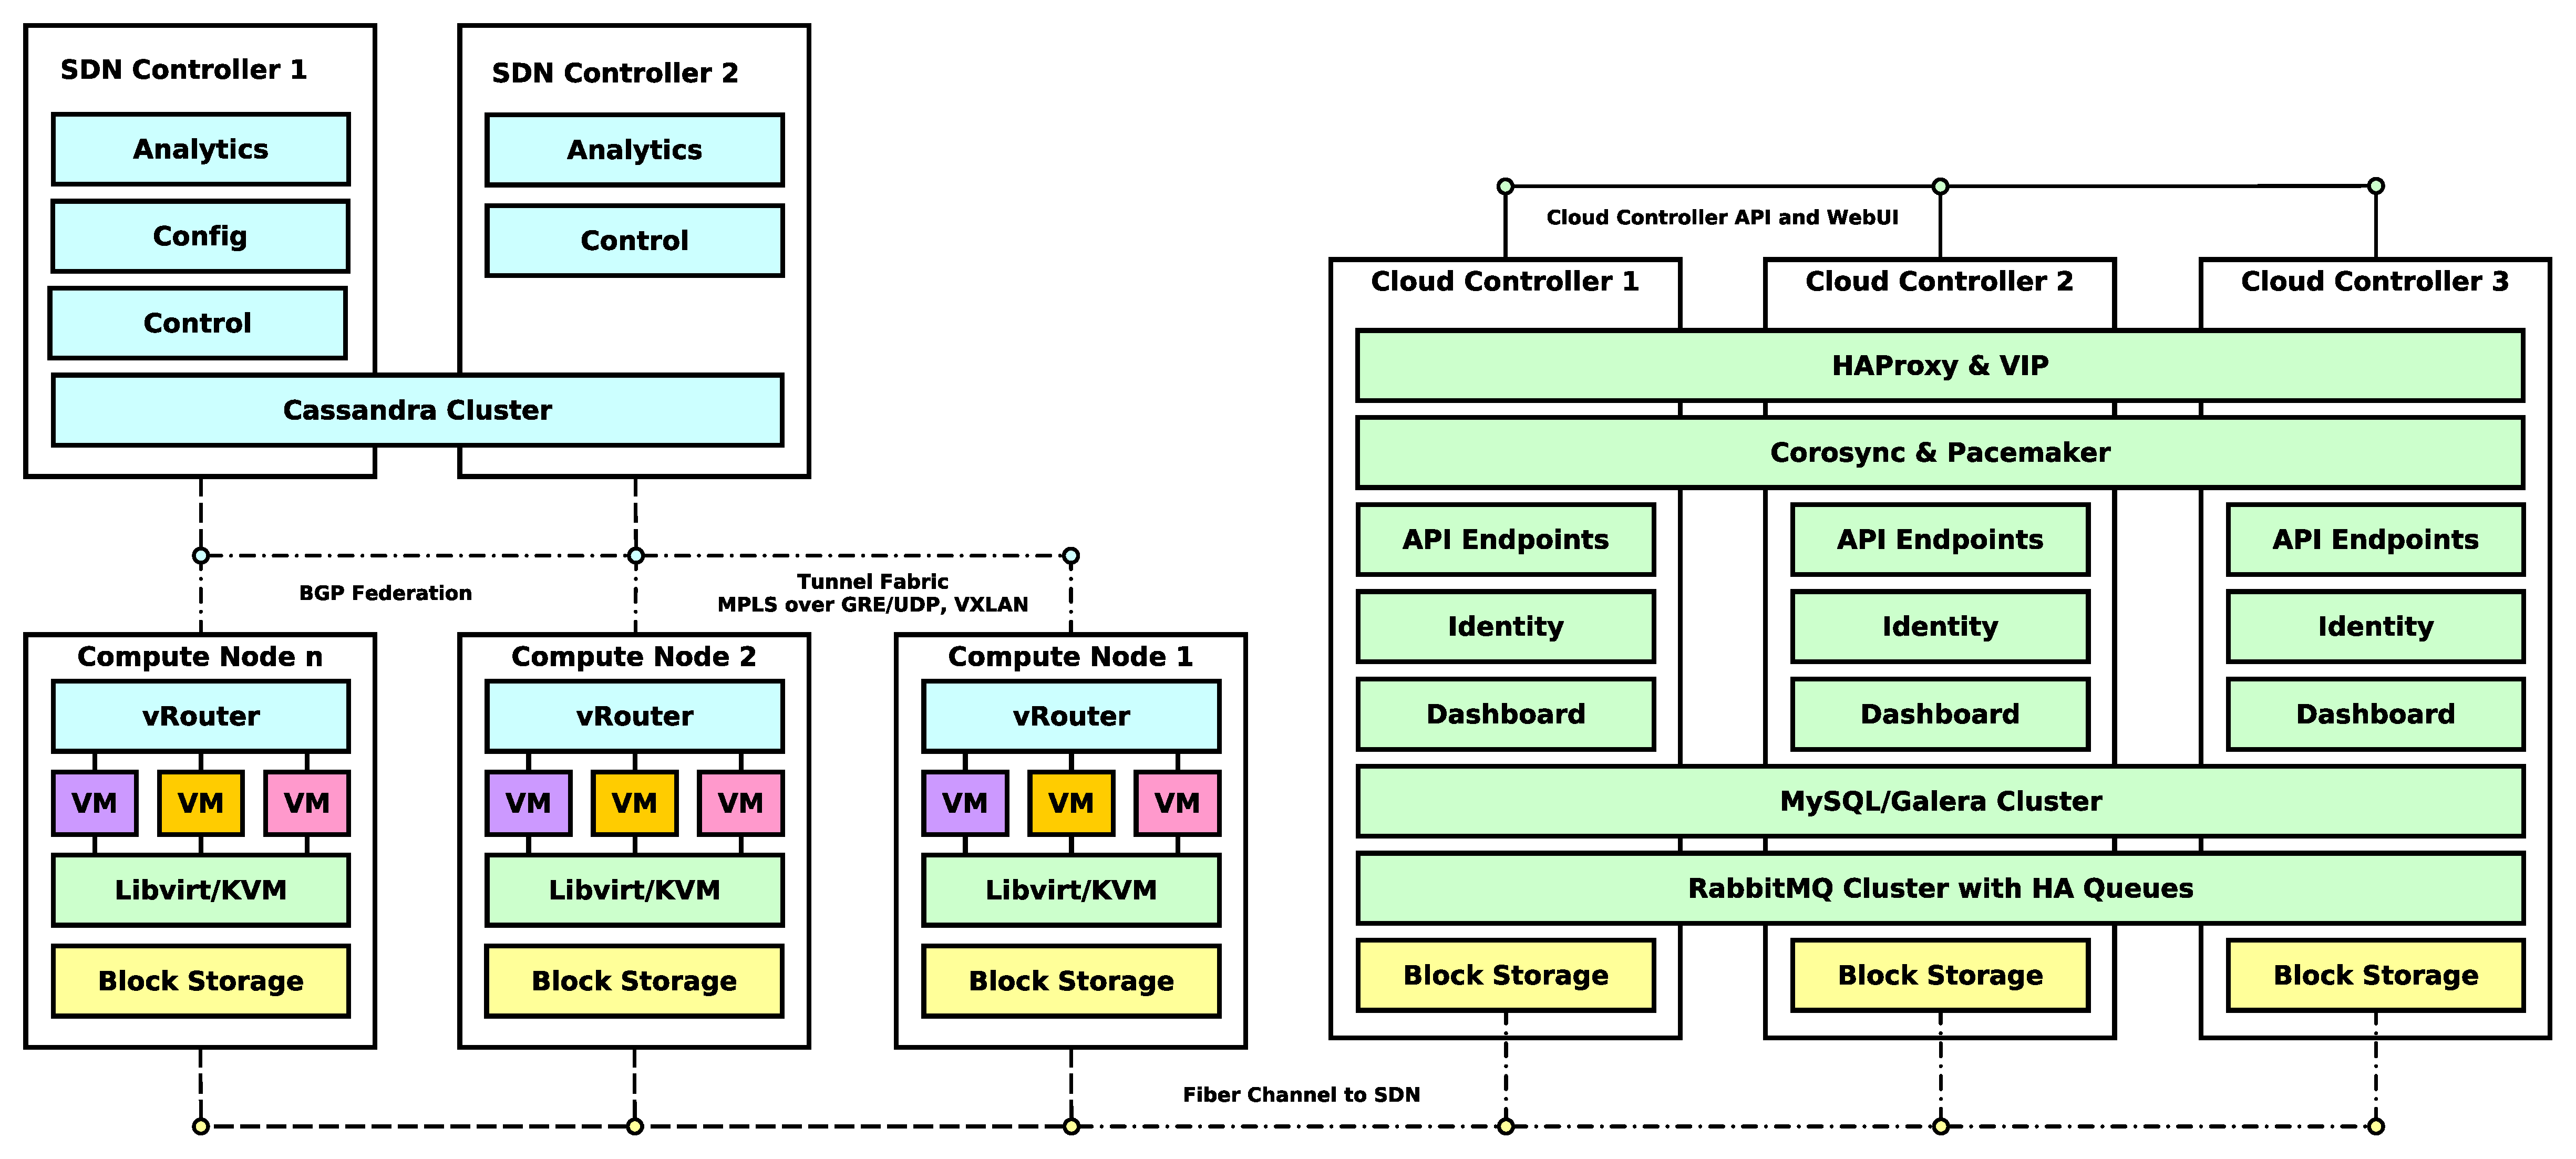
\includegraphics[scale=.15]{img/use_case_ha_sdn.eps}
\caption{Locality 2 Architecture}
\label{fig:pisek}
\end{figure}

%Jak funguje IaaS ve smyslu deploye masiny z pohledu controlleru - zavola scheduler, ten comupte, ten pak glance, pak pripadne cinder a neutron a pusti boot, kdyz to ma ready. a tim padem provoz.

Further versions of OpenStack introduce more complex services that use basic services to provide for example Data processsing, Database, Message Queue  or Orchestration. All services or modules within OpenStack architecture are independent and have pluggable backends or drivers. This allows vendors to develop plugin for their resources, that can be accessed and managed by the OpenStack API.

Fig. \ref{fig:modules} shows the core modules of OpenStack included in Icehouse release. Each module is briefly described including a serveral backends or plugins.


%Klasicky logicky model openstack architektury

%2) OpenStack architecture moduls

% Rozebrat services a představit modularitu a vendor plugins, drivers

\textbf{Identity - Keystone} is an OpenStack project that provides Identity, Token, Catalog and Policy services for use specifically by projects in the OpenStack family. 
\textit{Backends/plugins}: sql, ldap

\textbf{Image - Glance} service provides services for virtual disk images. Compute service uses image service to get the starting image of the virtual server.
\textit{Backends/plugins}: dir, Swift, Amazon S3

\textbf{Compute - Nova} service is designed to provision and manage large networks of virtual machines, creating a redundant and scalable cloud-computing platform. 
\textit{Backends/plugins}: KVM, Hyper-V, VMware vSphere, Docker

\textbf{Network - Neutron} is an OpenStack networking project focused on delivering networking as a service. It makes hard to deploy advanced networking services because of wide range of plugins.
\textit{Backends/plugins}: Nova flat networking, OpenVSwitch gre/vxlan, OpenContrail, VMware NSX, etc.

\textbf{Volume - Cinder} provides an infrastructure for managing volumes in OpenStack. It uses storage drivers for volumes direct mapping into virtual instances through FibreChannel or iSCSI. 
\textit{Backends/plugins}: LVM driver, SAN driver, EMC VNX, IBM Storwize, CEPH, Gluster, etc.

OpenStack is not only about its core services, but there are many services at infrastructural level that are essential as well.

\textbf{High Availability Cluster software} is responsible for clustering OpenStack services and creation High Availability in active/active or active/passive mode.
\textit{Backends/plugins}: corosync/pacemaker, keepalived

\textbf{Communication Service} is messaging between components of same OpenStack module.
\textit{Backends/plugins}: RabbitMQ, QPid, ZeroMQ

\textbf{Database Services} is responsible for storing persistent data of all modules.
\textit{Backends/plugins}: MySQL/galera, PostgreSQL

%Různé způsoby nasazení ukázky reálné architektury - promapovat ve 4 na ontologii

\subsection{USE CASES}

We participate in operations of several real OpenStack deployments in Central Eastern Europe. Each of them is different, which means that uses different backends in modules.
Because of lack of space we decided to show only one use case. Fig. \ref{fig:pisek} shows the logical architecture of TCP Virtual Private Cloud.

%\begin{figure}[!h]
%\centering
%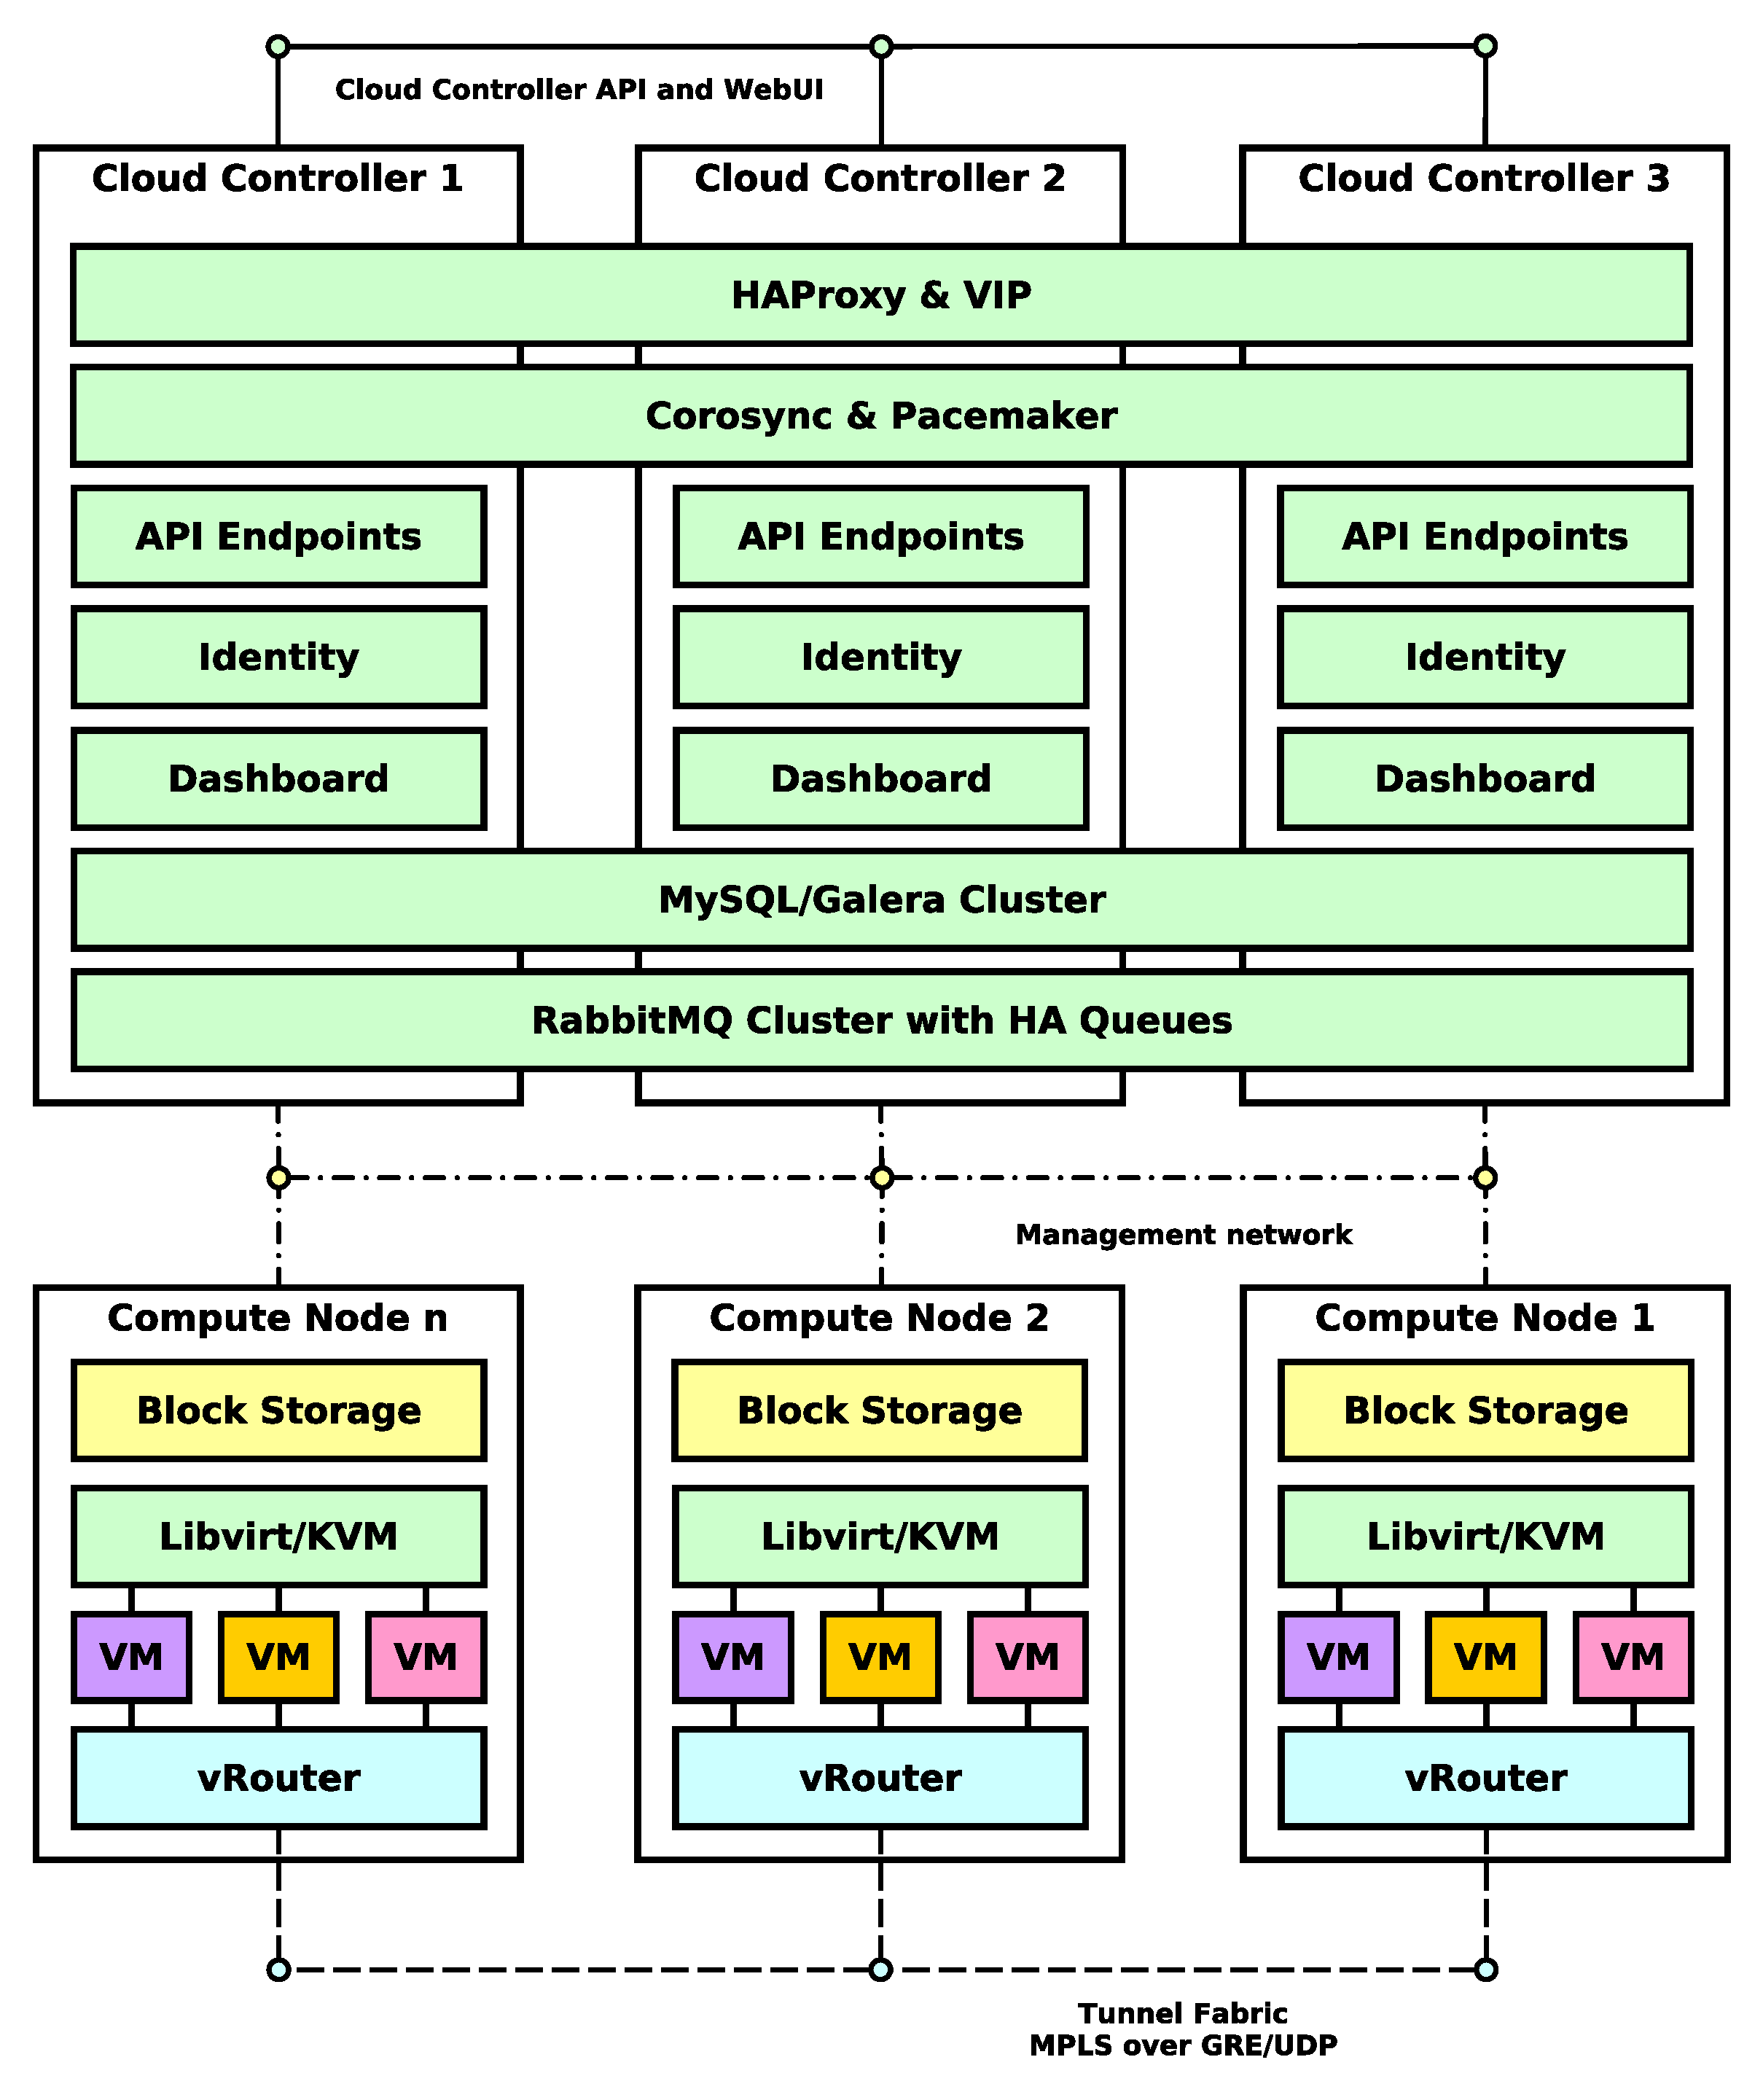
\includegraphics[scale=.2]{img/use_case_ha_gre.eps}
%\caption{Locality 1 Architecture}
%\label{fig:cm}
%\end{figure}

%\begin{figure}[!h]
%\centering
%\includegraphics[scale=.2]{img/use_case_l2_flat.eps}
%\caption{Locality 3 Architecture}
%\label{fig:cm}
%\end{figure}
